\section{Systemtest}
Den samlede systemtest foretages visuelt vha. test-projektet \textit{mic\_fht\_screen\_test}. 
Når projektet er downloadet til Arduinoen, ses det, at skærmen viser et output, som beskrevet i designet.
Det kan ses på figur \ref{fig:sys_test1}, hvor det ses, at indholdet i søjlerne er forskellige. 
For en demonstration af testen, sammen med lyd, henvises til den vedlagte video, $VIDEO_SOM_SKAL_HEDDE_NOGET_SMART$. 
Spektrogrammets output verificeres vha. et sweep, hvor det ses, at der forekommer aliasering på signalet harmoniske overtoner. 

\begin{figure}[H]
	\center
	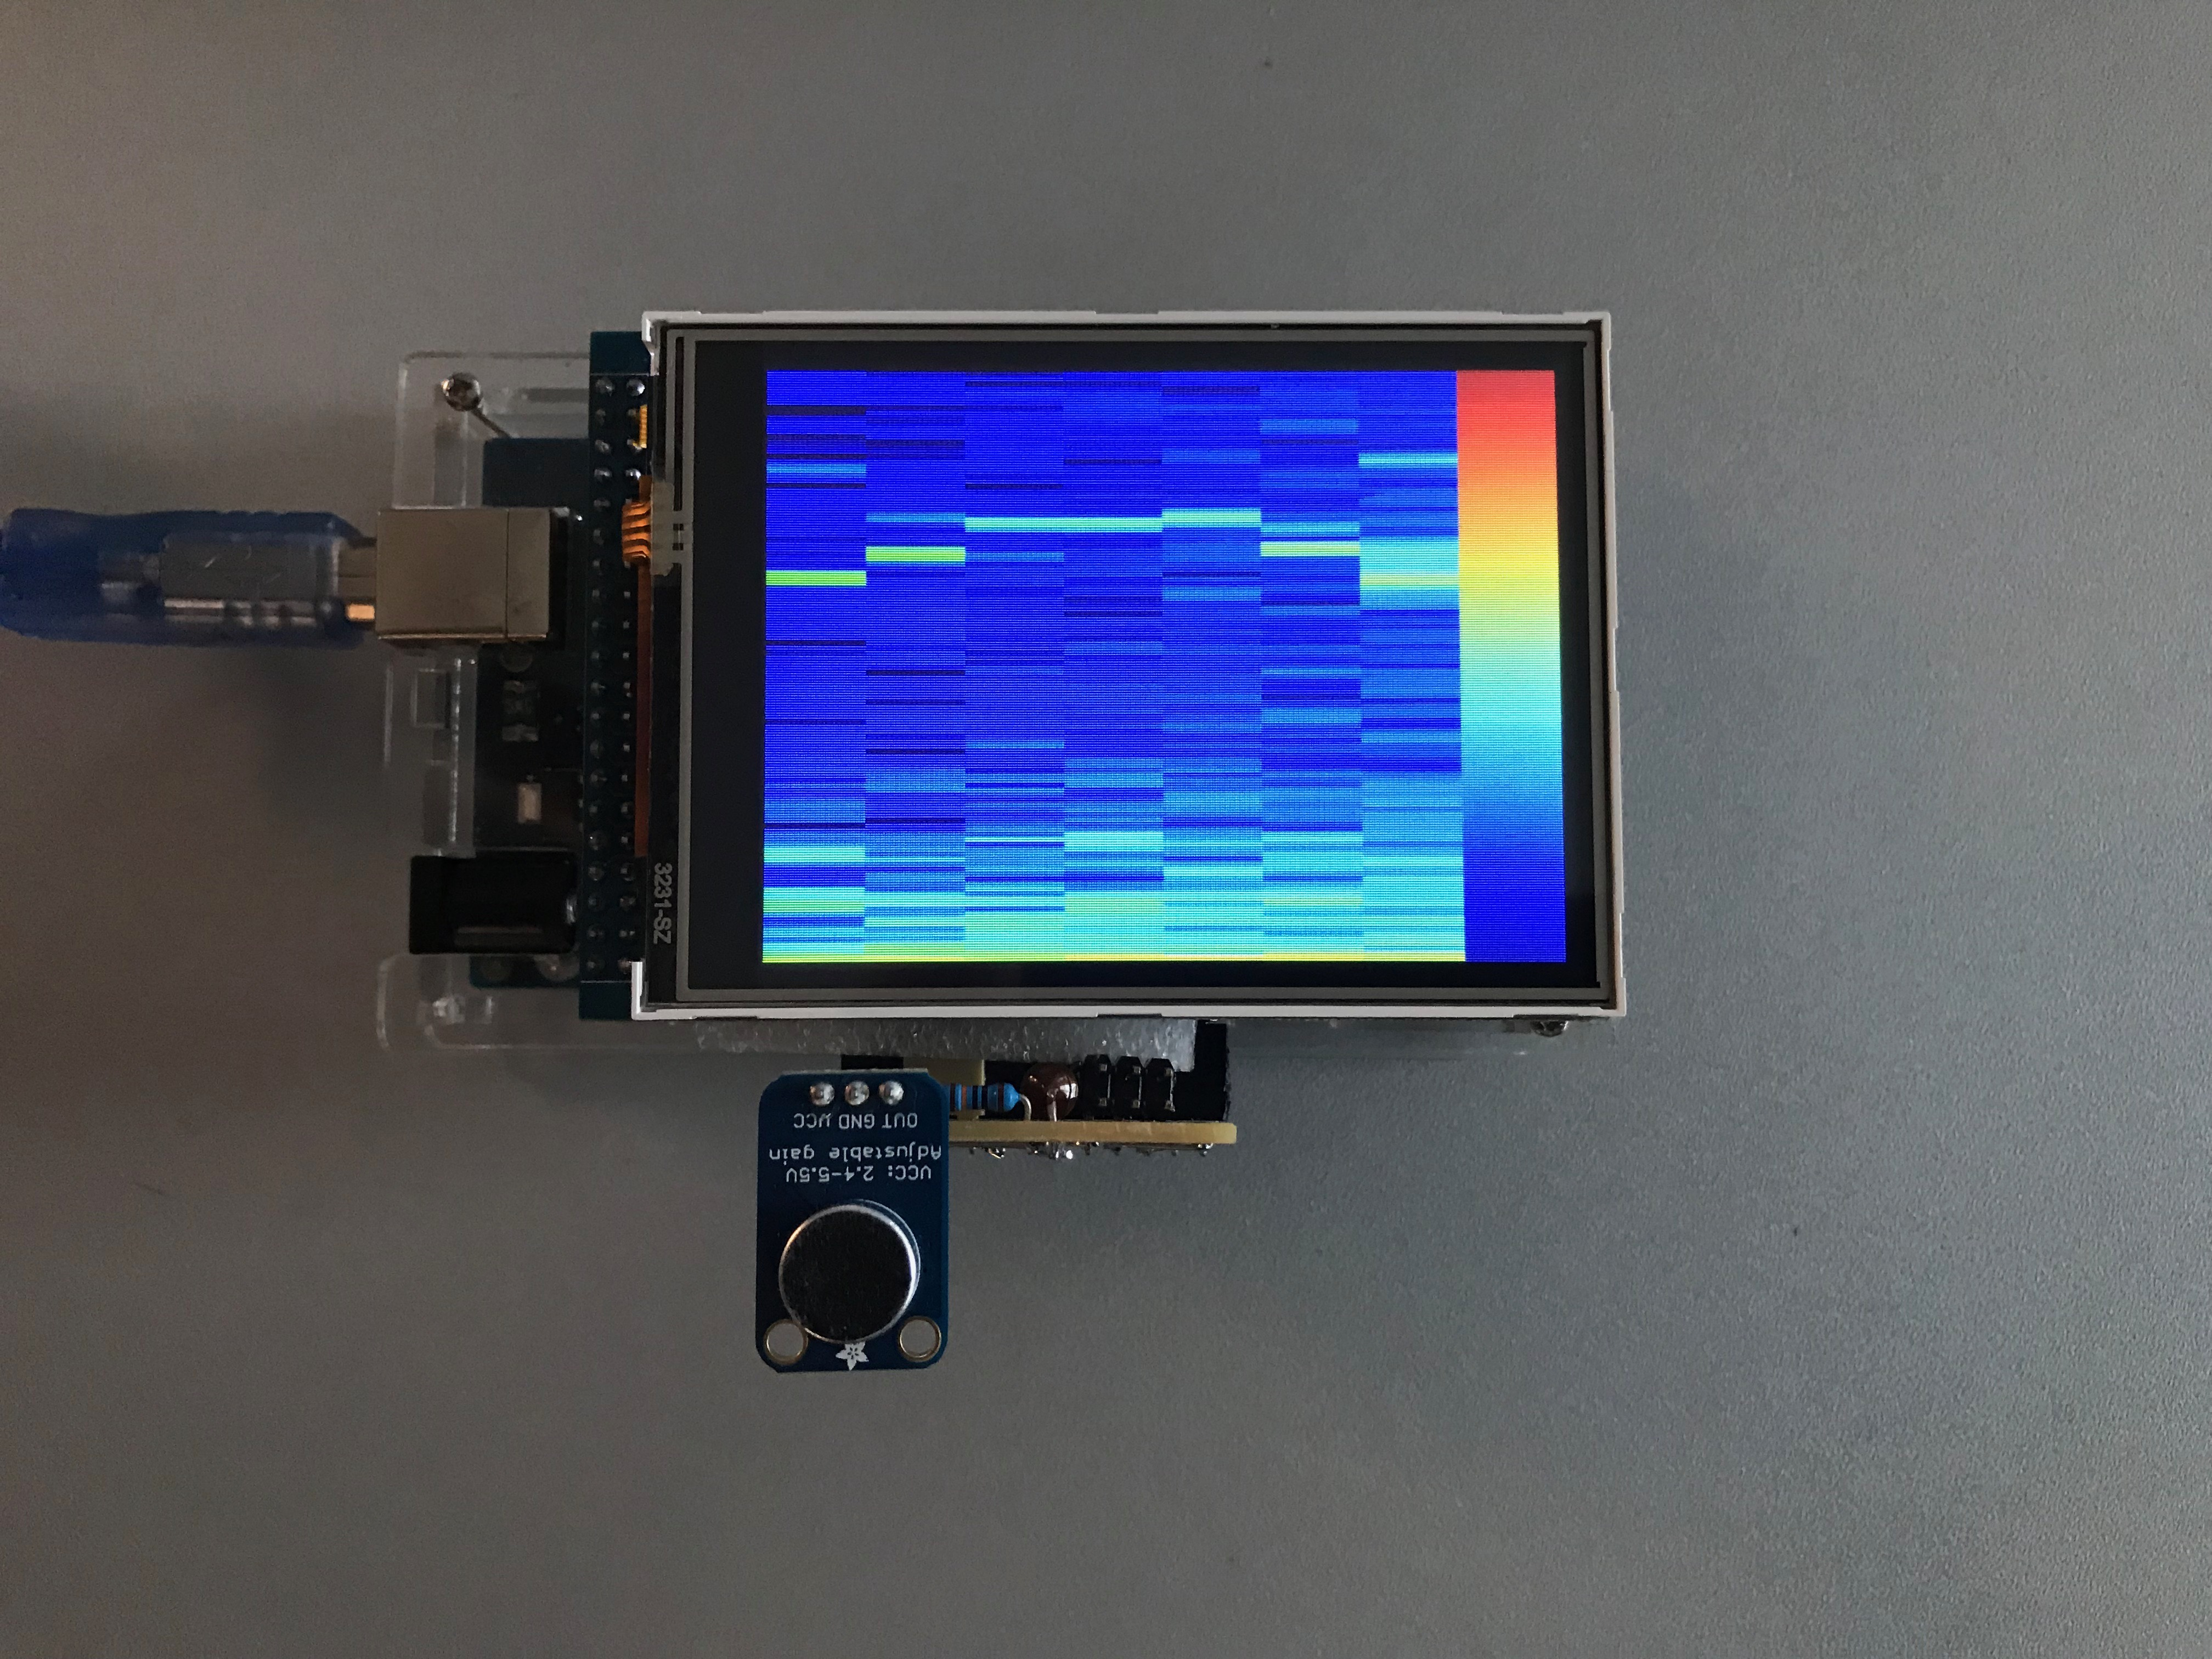
\includegraphics[width = 0.6\textwidth]{Figur/IMG_2470.JPG}
	\caption{Billede af den samlede systemtest}
	\label{fig:sys_test1}
\end{figure}